\chapter{Databasen}
Nedenfor følger design af software til databasen og dens interface. Dette er lavet på baggrund af kravspecifikation og systemarkitektur. 



\subsection{Modultes Ansvar}
Databasen er her hvor havne terminalens personale kan aflæse data fra skibet. Disse data er sendt fra KI. Programmerne indeholder brugergrænseflader der opfylder kravene, beskrevet i kravspecifikationen. Her kan der også ses en prototyper på brugergrænsefladen.
Database modulet har 3 dele. Severen, Web-siden og en mySQL database. \\
\textbf{Severen} står for kommunikationen immellem KI og Databasen. Severen modtager data fra KI og lager disse i en tekst fil\\
\textbf{Web-siden} giver brugeren mulighed for at se info om BROS samt at logge sig ind i BROS database hvorfra at data om skibe der er tilsluttet systemet kan aflæses. Web-sidens 3 vigtigste funktioner er at gemme ny data til mySQL databasen, slette den tekst fil som severen lavede og vise data for brugeren. For at håndtere web-sider der benytter sig af php (web-programmering) kræves der en web server som er i stand til at håndtere dette. En af de mest udbredte er apache serveren som også benyttes for denne webside.
\textbf{mySQL databasen} er en database som er  installeret på computeren. Alle data som er sendt fra KI er lageret i mySQL databasen.

\subsection{Klassediagrammer}
Nedenfor ses klassediagrammerne for databasen. Bemærk database modulet er lavet som en server del og en web del

\begin{figure}[htbp]
	\centering
	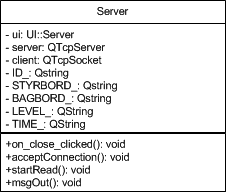
\includegraphics[width=0.4\textwidth]{billeder/serverKlassediagram}
	\caption{Klassedigram for databasens severer}
	\label{fig:serverKlassediagram}
\end{figure}

\begin{figure}[H]
	\centering
	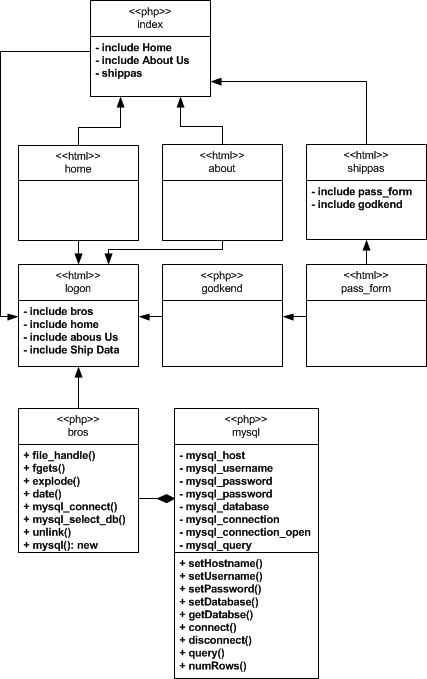
\includegraphics[width=0.5\textwidth]{billeder/web_klasse}
	\caption{Klassedigram for databasens web-side.}
	\label{fig:serverKlassediagram}
\end{figure}
\fxnote{check med kim, beskriv <<html>> og <<php>>}


\subsection{Globale variabler}


\subsection{Funktionsbeskrivelser}
\subsubsection{Server}
Denne header står for at starte serveren og starte GUI for korte informationer til brugeren. Alle informationer om server start, connection o datamodtagelse vil blive udskrevet her. 

\begin{table}[H]
\begin{tabular}{l p{12.5cm}}
\multicolumn{2}{l}{\texttt{\textcolor{blue}{Void} addLogEntry( \textcolor{blue}{QString} )}} \\
\hline
Står for at udskrive beskeder fra tcp klassen til GUI \\
Parametre: Ui::Server *ui;\\
Returværdi:&\\
\end{tabular}
\end{table}

\begin{table}[H]
\begin{tabular}{l p{12.5cm}}
\multicolumn{2}{l}{\texttt{\textcolor{blue}{Void} on\_closeServer\_clocked( )}} \\
\hline
Denne funktion håndtere luk knappen. Ved tryk knappen vil brugeren blive bedt om at svare ja eller nej til at lukke server connectionen \\
Parametre: Ingen\\
Returværdi:Ingen\\
\end{tabular}
\end{table}

\begin{table}[H]
\begin{tabular}{l p{12.5cm}}
\multicolumn{2}{l}{\texttt{\textcolor{blue}{Void} on\_webDatabase\_clicked( )}} \\
\hline
Denne funktion står for at håndtere den direkte adgang til den web baserede database. Ved tryk vil brugeren få åbnet et nyt vindue med database adgang \\
Parametre: QWebView* m\_pWebView\\
Returværdi:Ingen\\
\end{tabular}
\end{table}

\subsubsection{update}
Denne header står for at håndtere de struct's der benyttes til at at save data til log filen. 

\begin{table}[H]
\begin{tabular}{l p{12.5cm}}
\multicolumn{2}{l}{\texttt{\textcolor{blue}{Void} addLogEntry( \textcolor{blue}{QString} )}} \\
\hline
Står for at udskrive beskeder fra tcp klassen til GUI \\
Parametre: Ui::Server *ui;\\
Returværdi:&\\
\end{tabular}
\end{table}


\subsubsection{tcp}
Denne header står for tcp forbindelsen. Socket oprettes og connection adgang gives. Når data bliver modtaget blvier denne gemt i den eksterne log fil ship.txt

\begin{table}[H]
\begin{tabular}{l p{12.5cm}}
\multicolumn{2}{l}{\texttt{\textcolor{blue}{Void} addLogEntry( \textcolor{blue}{QString} )}} \\
\hline
Står for at udskrive beskeder fra tcp klassen til GUI \\
Parametre: Ui::Server *ui;\\
Returværdi:&\\
\end{tabular}
\end{table}

\begin{table}[H]
\begin{tabular}{l p{12.5cm}}
\multicolumn{2}{l}{\texttt{\textcolor{blue}{Void} acceptConnection( \textcolor{blue}{void} )}} \\
\hline
Beskrivelse:&Står for at acceptere forbindelse fra KI og connecte.\\
Parametre:&QTcpServer server\\
				&QTcpSocket* client\\
Returværdi:&\\
\end{tabular}
\end{table}

\begin{table}[H]
\begin{tabular}{l p{12.5cm}}
\multicolumn{2}{l}{\texttt{\textcolor{blue}{Void} startRead( \textcolor{blue}{void} )}} \\
\hline
Beskrivelse:&Læser data fra socket. Data til fil og GUI\\
Parametre:&QTcpSocket* client\\
Returværdi:&\\
\end{tabular}
\end{table}

\subsubsection{savedata}
Denne header står for at handtere lagring af data modtaget fra skibet. Den lager dataerne i ship.txt

\begin{table}[H]
\begin{tabular}{l p{12.5cm}}
\multicolumn{2}{l}{\texttt{\textcolor{blue}{int} save( \textcolor{blue}{save\_data} )}} \\
\hline
Står for at udskrive beskeder fra tcp klassen til GUI \\
Parametre: \\
Returværdi:&\\
\end{tabular}
\end{table}

\subsubsection{Wep-side}
Web-siden står for at fremvise skibs data grafisk for terminal personalet. Desuden står den for at lager data og loade data fra mySQL databasen.\\

\subsubsection{bros}

\begin{table}[H]
\begin{tabular}{l p{12.5cm}}
\multicolumn{2}{l}{\texttt{\textcolor{blue}{} file\_handle( \textcolor{blue}{} )}} \\
\hline
Beskrivelse:&Læse hvilken adresse databasen ligger på\\
Parametre:&\\
Returværdi:&\\
\end{tabular}
\end{table}

\begin{table}[H]
\begin{tabular}{l p{12.5cm}}
\multicolumn{2}{l}{\texttt{\textcolor{blue}{} fgets ( \textcolor{blue}{} )}} \\
\hline
Beskrivelse:&Læse hvilken adresse databasen ligger på\\
Parametre:&\\
Returværdi:&\\
\end{tabular}
\end{table}

\begin{table}[H]
\begin{tabular}{l p{12.5cm}}
\multicolumn{2}{l}{\texttt{\textcolor{blue}{} explode( \textcolor{blue}{} )}} \\
\hline
Beskrivelse:&Læse hvilken adresse databasen ligger på\\
Parametre:&\\
Returværdi:&\\
\end{tabular}
\end{table}

\begin{table}[H]
\begin{tabular}{l p{12.5cm}}
\multicolumn{2}{l}{\texttt{\textcolor{blue}{} date( \textcolor{blue}{} )}} \\
\hline
Beskrivelse:&Opdatere dato og tid når der gemmes til mySQL databasen\\
Parametre:&\\
Returværdi:&\\
\end{tabular}
\end{table}

\begin{table}[H]
\begin{tabular}{l p{12.5cm}}
\multicolumn{2}{l}{\texttt{\textcolor{blue}{} mysql\_connect( \textcolor{blue}{} )}} \\
\hline
Beskrivelse:&Læse hvilken adresse databasen ligger på\\
Parametre:&\\
Returværdi:&\\
\end{tabular}
\end{table}

\begin{table}[H]
\begin{tabular}{l p{12.5cm}}
\multicolumn{2}{l}{\texttt{\textcolor{blue}{} mysql\_select\_db( \textcolor{blue}{} )}} \\
\hline
Beskrivelse:&Læse hvilken adresse databasen ligger på\\
Parametre:&\\
Returværdi:&\\
\end{tabular}
\end{table}

\begin{table}[H]
\begin{tabular}{l p{12.5cm}}
\multicolumn{2}{l}{\texttt{\textcolor{blue}{} unlink( \textcolor{blue}{} )}} \\
\hline
Beskrivelse:&Læse hvilken adresse databasen ligger på\\
Parametre:&\\
Returværdi:&\\
\end{tabular}
\end{table}

\begin{table}[H]
\begin{tabular}{l p{12.5cm}}
\multicolumn{2}{l}{\texttt{\textcolor{blue}{new} mysql( \textcolor{blue}{} )}} \\
\hline
Beskrivelse:&Læse hvilken adresse databasen ligger på\\
Parametre:&\\
Returværdi:&\\
\end{tabular}
\end{table}

\subsubsection{mysql}
\begin{table}[H]
\begin{tabular}{l p{12.5cm}}
\multicolumn{2}{l}{\texttt{\textcolor{blue}{} setHostName( \textcolor{blue}{} )}} \\
\hline
Beskrivelse:&Læse hvilken adresse databasen ligger på\\
Parametre:&\\
Returværdi:&\\
\end{tabular}
\end{table}

\begin{table}[H]
\begin{tabular}{l p{12.5cm}}
\multicolumn{2}{l}{\texttt{\textcolor{blue}{} setUserName( \textcolor{blue}{} )}} \\
\hline
Beskrivelse:&Skriver brugernavn til databasen\\
Parametre:&\\
Returværdi:&\\
\end{tabular}
\end{table}

\begin{table}[H]
\begin{tabular}{l p{12.5cm}}
\multicolumn{2}{l}{\texttt{\textcolor{blue}{} setPassword( \textcolor{blue}{} )}} \\
\hline
Beskrivelse:&Skriver password til databasen\\
Parametre:&\\
Returværdi:&\\
\end{tabular}
\end{table}

\begin{table}[H]
\begin{tabular}{l p{12.5cm}}
\multicolumn{2}{l}{\texttt{\textcolor{blue}{} setDatabase( \textcolor{blue}{} )}} \\
\hline
Beskrivelse:&Fortæller mySQL hvilken database der skal benyttes\\
Parametre:&\\
Returværdi:&\\
\end{tabular}
\end{table}

\begin{table}[H]
\begin{tabular}{l p{12.5cm}}
\multicolumn{2}{l}{\texttt{\textcolor{blue}{} getDatabase( \textcolor{blue}{} )}} \\
\hline
Beskrivelse:Tager fat i databasen\\
Parametre:&\\
Returværdi:&\\
\end{tabular}
\end{table}

\begin{table}[H]
\begin{tabular}{l p{12.5cm}}
\multicolumn{2}{l}{\texttt{\textcolor{blue}{} connect( \textcolor{blue}{} )}} \\
\hline
Beskrivelse:&Står for at samle localhost, username, password, database og connecte til databasen\\
Parametre:&\\
Returværdi:&\\
\end{tabular}
\end{table}

\begin{table}[H]
\begin{tabular}{l p{12.5cm}}
\multicolumn{2}{l}{\texttt{\textcolor{blue}{} disconnect( \textcolor{blue}{} )}} \\
\hline
Beskrivelse:&Lukker database forbindelsen\\
Parametre:&\\
Returværdi:&\\
\end{tabular}
\end{table}

\begin{table}[H]
\begin{tabular}{l p{12.5cm}}
\multicolumn{2}{l}{\texttt{\textcolor{blue}{} query( \textcolor{blue}{} )}} \\
\hline
Beskrivelse:&Opretter database kø og skriver data til skærm\\
Parametre:&\\
Returværdi:&\\
\end{tabular}
\end{table}

\begin{table}[H]
\begin{tabular}{l p{12.5cm}}
\multicolumn{2}{l}{\texttt{\textcolor{blue}{} numRows( \textcolor{blue}{} )}} \\
\hline
Beskrivelse:&Checker hvor mange rækker der findes i databasen bruges desuden til at udskrive om databasen er tom.\\
Parametre:&\\
Returværdi:&\\
\end{tabular}
\end{table}

\section{Design}
\subsection{Server}
\begin{figure}[htbp]
	\centering
	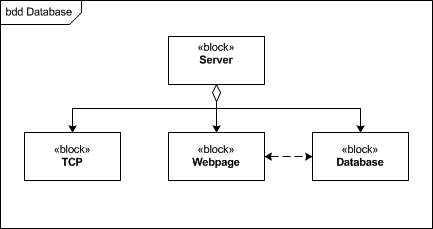
\includegraphics[width=0.6\textwidth]{billeder/bdd_server}
	\caption{BDD server}
	\label{fig:bdd_server}
\end{figure}






